% LaTeX file for Chapter 01


\chapter{Introduction}

\section{RNA sequencing}
RNA sequencing (RNA-seq) is a technology for detecting and quantifying the mRNA molecules of a biological sample \citep{rna_seq}. The invention of RNA-seq was a major breakthrough in the field of bioinformatics that replaced the use of microarray technology in the late 00's. In comparison to microarrays, RNA-seq allows for full sequencing of the whole transcriptome whereas microarrays only profile predefined transcripts through hybridization \citep{rna_seq_comparison}. Further, various protocols have since been derived from the standard RNA-seq protocol, e.g. single-cell RNA sequencing \citep{rna_seq}.

\subsection{Bulk RNA-seq}
Bulk RNA sequencing allows detecting an aggregated signal across a mixture of cells. There are many applications for bulk RNA-seq. For example, it can be used to study the differences of expression profiles between tissues in healthy vs disease or across treatments \citep{rna_seq}. However, with bulk RNA-seq one can only estimate the average expression of each gene across a population of cells without regard for the differences between cell types. RNA-seq has several use cases. It can be used to study which genes are turned on in a cell and what their level of transcription is. This allows researchers to understand the biology of a cell at a deeper level. Further, RNA-seq allows the identification of variants and allele specific expression. It is also possible to study the patterns of alternative splicing, which are important to understand their contribution to cell differentiation and human disease.

\subsection{Single-cell RNA-seq}
Single-cell RNA sequencing was developed to overcome some of the limitations of bulk RNA sequencing. With scRNA-seq it is possible to estimate the distribution of expression levels for each gene across a population of cells. This allows answering new biological questions where cell-specific characteristics are important. However, there are some caveats with scRNA-seq \citep{scrna_seq}. scRNA-seq data in general is much more variable than bulk RNA-seq data due to both higher biological and technical variability at single-cell level \citep{scrna_seq}. Figure \ref{fig:SC_RNA} shows the typical workflow of a scRNA-seq experiment. Said workflow is broadly summarized by the following steps:

\begin{enumerate}
   \item RNA extraction
   \item Reverse transcription into cDNA
   \item Adapted ligation
   \item Amplification
   \item Sequencing
   \item Downstream analysis using bioinformatics tools
\end{enumerate}

\begin{figure}[!htb]
\begin{center}
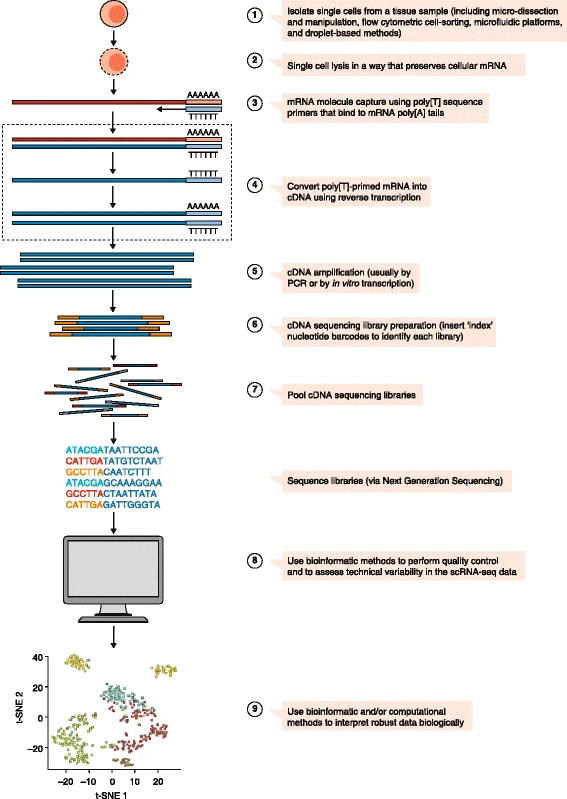
\includegraphics{../figures/scrna_protocol.png}
\end{center}
\caption{General workflow of single-cell RNA-sequencing experiments \citep{scrna_seq}}
\label{fig:SC_RNA}
\end{figure}
\FloatBarrier

\subsection{Quantification of single-cell RNA-seq data}
scRNA-seq data has distinct characteristics that prevent it from being processed by widely used tools developed for bulk RNA-seq data \citep{alevin_fry}. In general, quantification works by aligning the reads generated from the RNA-seq to the reference genome. There are several tools that allow to do that, notably: \emph{STAR} \citep{star}, \emph{kallisto | bustools} \citep{kallisto} and \emph{alevin} \citep{alevin}. However, there is a difference between the first tool and the other two. STAR is an aligner, whereas the other two tools are mapping tools (pseudo-aligners). The difference between an full-aligner and a mapping tool is that the latter does not look for the exact location of the read, as a consequence pseudo-alignment is much faster than full-alignment. Here we focus on \emph{alevin-fry}, and the method we have developed, which will be introduced later, has been built to work on the output of \emph{alevin-fry}.

\section{Objective}

\subsection{RNA velocity}
We investigate spliced and unspliced reads from scRNA-seq data. During transcription, DNA is decoded into precursor messenger RNA (pre-mRNA). Pre-mRNA contains both coding (exons) and non-coding regions (introns). In a next step, introns are removed from the pre-mRNA which leaves only the mature mRNA. Figure \ref{fig:RNA_VELO} shows the process from DNA to mature mRNA, where $\alpha$ is the transcription rate, $\beta$ is the splicing rate and $\gamma$ is the degradation rate.

\begin{figure}[!htb]
\begin{center}
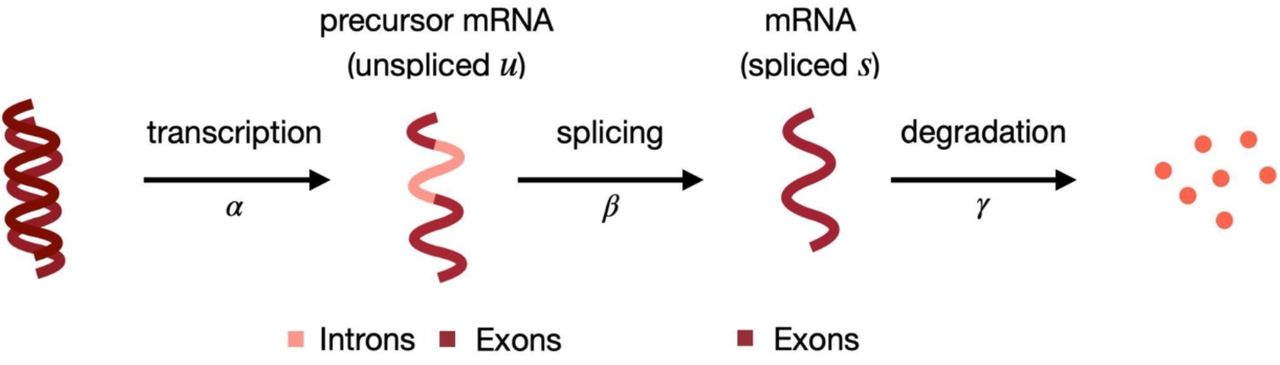
\includegraphics{../figures/regulation.jpg}
\end{center}
\caption{The transcription process from DNA to mature mRNA \citep{rna_velo_traj}}
\label{fig:RNA_VELO}
\end{figure}
\FloatBarrier

It was assumed that there is a signal (RNA velocity) detectable in scRNA-seq data that could reveal the rate and direction of change of an entire transcriptome \citep{rna_velo}. To quantify the relationship between the abundance of pre-mRNA and mature RNA, a simple system of ordinary differential equations was assumed (\ref{eqn:RNA_VELO}): The solution of said system at equilibrium can then easily be estimated and used to explore the regulation of genes:

\begin{equation}
\begin{array}{l}
\frac{du}{dt} = \alpha - \beta u \\
\frac{ds}{dt} = \beta u - \gamma s
\end{array}
\label{eqn:RNA_VELO}
\end{equation}

The derivative of the spliced counts is then defined as the RNA velocity of cells. Thus, the balance of spliced and unspliced counts allows estimating whether a gene is up- or downregulated. If a larger fraction of unspliced counts are present than expected at equilibrium, a gene is likely upregulated. This is because within a short time interval, the newly spliced mRNA will exceed the amount of spliced mRNA which is degraded. Contrarily, if more spliced counts are present at equilibrium than expected, a gene is likely downregulated.

\subsection{Differential regulation}
The abundance of spliced and unspliced reads is directly linked to the regulation of genes and RNA velocities \citep{rna_velo}. Our idea is to examine how the abundance of spliced and unspliced counts changes between experimental conditions and biological replicates. We translate this intuition into the comparison of two experimental conditions, e.g. healthy vs. disease. Following the same intuitive rationale of RNA velocity, if a gene has a higher abundance of unspliced (spliced) counts in group A  compared to group B, then this gene is likely being up-regulated (down-regulated) in group A compared to group B. Thus, we explore the differences in abundance of spliced and unspliced counts to study the differences in regulation between experimental conditions.

If the data contains multiple cell clusters (e.g. cell types), similarly to differential state analyses (\cite{muscat} and \cite{distinct}) we will perform differential analyses in each cluster of cells, hence identifying cell-cluster/cell-type specific changes between conditions. The idea of performing differential analyses on the abundance of spliced and unspliced or exonic and intronic reads is not completely novel as there are at least two other methods that achieve that: \emph{eisaR} and \emph{BRIE2}.

\subsection{Existing methods}

\textbf{eisaR} \citep{eisar_package} is a R package implementation that allows for the split analysis between exons and introns. It allows one to measure changes in mature RNA and pre-mRNA across different experimental conditions. Ultimately, \emph{eisaR} differential testing is based on edgeR \citep{edger_package}. edgeR is a R package that performs differential expression analyses between groups of samples. It implements statistical methods that are based on the negative binomial distribution as a model for count variability. \\

\noindent \textbf{BRIE2} \citep{brie2} is a Bayesian hierarchical model that is implemented in Python and supports the analysis of splicing processes between spliced and unspliced RNA. There are two modes in which the tool can be used. First, the use of differential alternative splicing (DAS), where the aim is to quantify the proportions of alternative splicing isoforms. Second, the use of differential momentum genes (DMG), where the objective is to quantify the proportions of spliced and unspliced RNA in each gene and each cell.

Originally, \emph{eisaR} and \emph{BRIE2} were developed to analyse all cells, but can easily be adapted to perform cell-type specific differential analyses.

\subsection{Mapping uncertainty}
We can identify two main sources of mapping uncertainty concerning spliced and unspliced reads: i) multi-mapping reads across spliced and unspliced versions of a gene, and ii) reads compatible with multiple genes. In fact, it has been shown that many reads (5-40\%) map to multiple genes (\cite{mapping1}, \cite{mapping2}). In our real data analyses (see Section 3), we found approximately 20-30\% of such multi-mapping reads across genes. We additionally found that a significant fraction of reads (6-19\%) are compatible with both S and U versions of a gene. Therefore, the estimated spliced and unspliced counts carry a substantial amount of uncertainty, which should be accounted for in downstream analyses. However, both \emph{eisaR} and \emph{BRIE2} use estimated spliced and unspliced counts and neglect the mapping uncertainty. In this thesis, we propose two approaches that account for said mapping uncertainties.
